\chapter{Entwicklung}
\label{cha:Entwicklung}

Die im zweiten Kapitel beschriebenen theoretischen Grundlagen und auch praktischen Überlegungen zur Implementierung verteilter Systeme für Drohnenschwärme müssen jetzt in der Form eines Prototypen umgesetzt werden. Dies beginnt mit der Beschreibung der getroffenen Annahmen, da die Implementierung eines voll funktionsfähigen verteilten Systems in begrenzten Zeitrahmen mehr Zeitaufwand, Testing und Aufmerksamkeit für Details erfordert hätte. Dann folgt die Beschreibung des Gesamtsystems mit einer Gliederung der wichtigsten Komponenten. Anschließend wird die Implementierung des Raft-Algorithmus detailliert untersucht.

\section{Annahmen und Einschränkungen in der Entwicklung}

Die Implementierung jedes Systems erfordert Zeit, die auch exponentiell mit der Komplexität des Vorhabens steigt. Um einen realisierbaren Prototypen innerhalb einer überschaubaren Zeit zu implementieren, wurde eine Reihe von Annahmen getroffen.

\subsection{Scala als Programmiersprache}

Als Programmiersprache für die Implementierung des Prototypen wurde Scala verwendet. Scala ist eine \textit{Universalsprache}, die sowohl objektorientierte Programmierung als auch funktionale Programmierung unterstützt. Die Sprache ist statisch typisiert. Der Scala-Quellcode wird in Java Bytecode kompiliert, sodass der resultierende ausführbare Code auf der Java Virtual Machine (JVM) ausgeführt werden kann. Scala bietet Interoperabilität mit Java. Im Gegensatz zu Java verfügt Scala über viele Eigenschaften funktionaler Programmiersprachen, wie beispielsweise Scheme, Standard ML und Haskell, einschließlich Currying, Immutability (Unveränderlichkeit), die Lazy Evaluation (bequeme oder auch faule Auswertung) und Pattern Matching. Es verfügt ebenfalls über ein fortschrittliches Typsystem, das algebraische Datentypen, Kovarianz und Kontravarianz sowie anonyme Typen unterstützt. Andere Funktionen von Scala, die in Java nicht vorhanden sind, sind das Überladen von Operatoren, optionale Parameter und benannte Parameter.

Laut \textit{"Github Language Stats"} (Stand 23.12.2020) erreichte Scala bei der Anzahl an Pull-Requests den elften Platz und überholte somit Programmiersprachen wie Rust, Kotlin, Swift und Haskell.

Für die Implementierung eines Produktivsystems, welches auf einer Drohne läuft und auch Leistungsanforderungen des Betriebssystems einer Drohne erfüllt, wären solche Systemprogrammiersprachen wie C++ oder Rust geeignet. Scala ermöglicht aufgrund seiner Simplizität ein schnelles Prototyping, das Aktorsystem (actors system) dieser Programmierungssprache mit zahlreichen Eigenschaften hat einen guten Ruf bekommen und die Integration des Aktorsystems mit dem Play-Web-Frameworks machen Scala zu einer guten Option für die Implementierung eines Prototypen.

\subsection{Akka für das Implementieren verteilter Systeme}

Den größten Vorteil von Scala bietet das Aktorsystem, genauer gesagt das Aktorsystem der Akka-Bibliothek. Die Verwendung von Akka macht die Erstellung der Infrastruktur für ein Aktorsystem und das Schreiben des Low-Level-Codes, der zur Steuerung des grundlegenden Verhaltens erforderlich ist, überflüssig.

Ein Aktor in Akka hat immer einen Elternknoten und alle Knoten sind Kinder des Guardian-Knotens, der beim Start eines Aktorsystems erstellt wird. Eine Instanz des ActorSystems dient zur Kommunikation mit dem Aktorsystem, zur Erstellung neuer Aktoren, zur Adressierung und zur Verwaltung des Kontexts. Eine reibungslose Kommunikation zwischen den Aktoren ist nur innerhalb des Systems möglich. Wenn eine andere Softwarekomponente einen Aktor innerhalb des Aktorsystems aufrufen möchte, muss diese Anfrage mittels Adapter übersetzt werden. Dasselbe gilt für Antworten des Aktorsystems. Die Kommunikation im Aktorsystem ist immer asynchron.

Bevor der erste Aktor gestartet wird, hat Akka bereits 2 Aktoren erstellt. Die Namen dieser eingebauten Aktoren enthalten \textit{"guardian"} (Wächter). Die Guardian-Aktoren umfassen:

\begin{enumerate}
	\item "/" - der sogenannte Root-Guardian. Das ist das übergeordnete Element aller Aktoren im System und das letzte, das angehalten wird, wenn das System stoppt.
	
	\item "/system" - der System-Guardian. Das ist ein Aktor, der das System aufrechterhält. Akka oder andere Bibliotheken, die auf Akka basieren, können Aktoren im Systemnamespace erstellen.
	
	\item "/user " - der Benutzer-Guardian. Das ist der Aktor, der alle anderen Aktoren einer Anwendung startet.
\end{enumerate}

Struktur der Guardian Aktoren wird in der Abbildung \ref{fig:akkaActors} dargestellt.

\begin{figure}
	\centering
	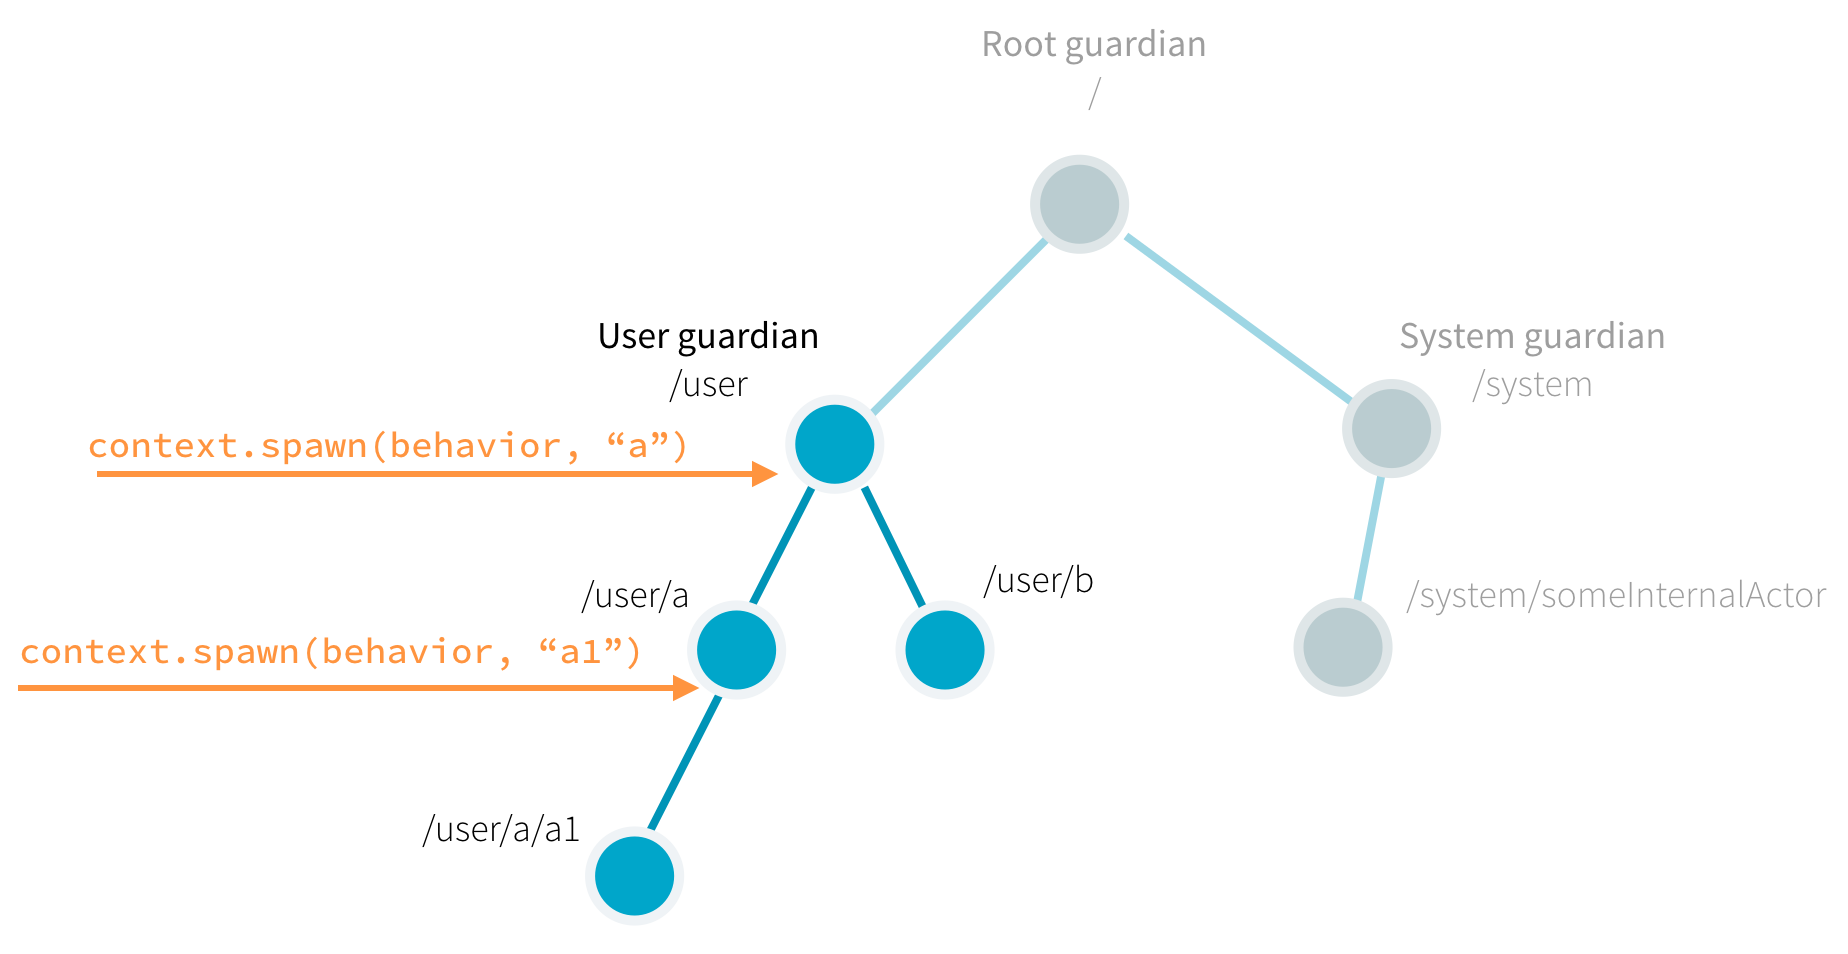
\includegraphics[width=0.7\linewidth]{images/3_akka_actors}
	\caption{Beispiel eines Aktorsystems zusammen mit den Aktoren, die von Akka standardmäßig erstellt werden.}
	\label{fig:akkaActors}
\end{figure}

Anwendung des Akka Aktorsystems und seiner Module bringt folgende Vorteile für verteilte Systeme:

\begin{description} 
	\item[Protokollunabhängigkeit.] Standardmäßig bietet Akka eine Integration mit HTTP, aber mittels Konnektoren (Adapters anders gesagt) kann man auch problemlos über MQTT, AMQP, JMS (Java Message Service) und gRPC kommunizieren.
	
	\item[Verteilte Aktoren.] Akka Remoting ermöglicht Aktoren, die auf verschiedenen Rechnern laufen, Nachrichten nahtlos auszutauschen. Dank des Aktormodells sieht ein ferner und lokaler Nachrichtenversand gleich aus. Es bietet die Basis, auf der das Cluster-Subsystem aufgebaut ist.
	
	\item[Unterstützung von Clusters.] Wenn es in einem verteilten System eine Reihe von Aktoren gibt, die zusammenarbeiten, um eine Aufgabe zu lösen, muss das System auf eine bestimmte Weise aufgebaut und gesteuert werden. Während Akka-Remoting das Problem der Adressierung und Kommunikation zwischen Komponenten eines verteilten Systems löst, bietet Clustering die Möglichkeit, diese Knoten in der Form eines Metasystems mit einem Mitgliedschaftsprotokoll zu organisieren. Das ist ein Teil der Kontrollebene eines Clusters.
	
	\item[Sharding (horizontale Fragmentierung).] Sharding ist ein Vorgehen, das verwendet wird, um eine große Anzahl von Aktoren auf Knoten eines Clusters aufzuteilen und sie auch auf andere Knoten zu verschieben, wenn andere Knoten abstürzen oder unerreichbar werden.
\end{description}

Akka verfügt über mehrere Kommunikationspatterns. Einige von ihnen sind für Aktorsysteme spezifisch und dienen dazu, ein erklärbares und skalierbares System zu entwickeln. Diese spezifische Patterns sind z.B:

\begin{enumerate}
	\item Zusendung des Ergebnisses eines Futures \footnote{Ein Future bezeichnet einen Platzhalter (Proxy) für ein Ergebnis, das noch nicht bekannt ist, meist weil seine Berechnung noch nicht abgeschlossen ist.} an sich selbst
	
	\item Per-Session-Child-Actor (Erstellung eines Aktors je Sitzung) in dem ein Elternknoten einen Kindknoten erstellt. Der Kindknoten stellt eine asynchrone Operation dar, die allen anderen Aktoren abfragen muss, das Ergebnis dem Elternknoten zur Verfügung stellt und sich anschließen stoppt. Die Erstellung eines neuen Aktors für jede Anfrage kann verschwenderisch klingen (vor allem in einem eingebetteten System), die Erstellung eines neuen Aktors erfordert allerdings keine Ressourcen des Betriebssystems und ist deswegen sehr billig.
\end{enumerate}

Patterns, die bei der Implementierung des Raft-Algorithmus eingesetzt wurden, sind:

\begin{description} 
	\item[Fire and Forget (Tell-Ansatz).] Fire-And-Forget ist der fundamentale Weg für die Kommunikation zwischen Aktoren. "Tell" ist asynchron, was bedeutet, dass die Methode in einem anderen Thread gestartet wird. Nachdem der Befehl ausgeführt wurde, gibt es keine Garantie, dass die Nachricht noch vom Empfänger verarbeitet wurde. Das bedeutet auch, dass es keine Möglichkeit gibt herauszufinden, ob die Nachricht empfangen wurde, die Verarbeitung erfolgreich war oder fehlgeschlagen ist. Fire-And-Forget ist so üblich bei Akka, dass es einen speziellen symbolischen Namen hat: “!” (Ausrufezeichen). Der Versand einer Nachricht hätte dann so ausgesehen “actor ! message”.
	
	\item[Request-Response mit einer oder mehreren Antworten.] Mehrere Interaktionen erfordern eine oder mehrere Antworten. Um die Antwort zu erhalten muss der Absender seine Adresse in der Nachricht mitschicken.
	
	\item[Request-Response mit einer einzelnen Antwort (Ask-Ansatz).] Wenn für eine Anfrage genau eine Antwort erwartet wird, verwendet man Ask-Anfragen. Eine Ask-Anfrage hat ebenfalls eine spezielle Bezeichnung: “?”. Da alle Kommunikationen im Aktorsystem asynchron sind, darf man einen Aktor mit der Ask-Anfrage nicht blockieren. Die Antwort wird asynchron empfangen und in einen Callback übergeben, der bei der Absendung der Ask-Anfrage erstellt sein soll.
	
	\item[Interaktion mit externen Komponenten.] Da Aktoren standardmäßig nur mit anderen Aktoren innerhalb eines Aktorsystems kommunizieren können, braucht man eine Brücke für die Außenwelt. Eine der möglichen Lösungen ist Future. Dies ist eine Abstraktionsschicht über übliche Callbacks und stellt Ergebnis einer asynchronen Operation dar. Ein Future wird normalerweise von einem Promise erstellt, der ein Proxy zwischen einer Rechenoperation und dem Future (dem asynchronen Ergebnis) darstellt.
	
	\item[Scheduling messages to self (Zusendung an sich selbst zu planen).] Standardmäßig erlaubt Akka einem Aktor Nachrichten an sich selbst zu schicken. Dadurch kann man Timeouts implementieren, auf denen Paxos und andere Algorithmen für verteilte Systeme beruhen.
\end{description}

Das Kommunikationsmuster eines Knotens mit anderen Knoten und dessen Verhalten kann sich mit der Zeit ändern. Das passiert, wenn ein Knoten mehr Funktionen bzw. andere Funktionen in der Hierarchie übernimmt, beispielsweise die Funktion eines Beobachters und Workers gleichzeitig, oder die Funktion eines Beobachters und eines Response Aggregators. Da ein Aktor als solcher einen Zustandsautomaten darstellt, der beliebig kompliziert sein kann, führt es zu einem Zustandsautomaten mit verschachtelten Zuständen. Um diese Überlappung von Funktionen und Komplexitäten aufzulösen, gibt es bei Akka zwei Herangehensweisen: die erste klassische Methode, die sich vorzüglich bewährt hat, ist die Zersetzung eines Aktors in mehrere Aktoren. Die zweite Methode ist die Auswechslung von \textit{Behaviors} (Verhalen). Ein Behavior repräsentiert einen Übergang in einen neuen globalen Zustand. Ein solcher globaler Übergang wäre in Raft der Übergang vom Follower-Zustand zum Leader-Zustand. Ein Aktor dient in diesem Fall als Container (Behälter) für Behaviors mit einem anfänglichem Verhalten. Behaviors entscheiden selbstständig, was das nächste Behavior ist und ob ein Behavior zu einem bestimmten Zeitpunkt überhaupt ausgetauscht werden soll. Wenn ein Behavior ausgewechselt wird, bleibt der Container (also Aktor) intakt. Einen Übergang von Zuständen innerhalb eines Aktors könnte man beim Raft-Algorithmus wie in der Abbildung \ref{fig:stateTransition} darstellen.

\begin{figure}
	\centering
	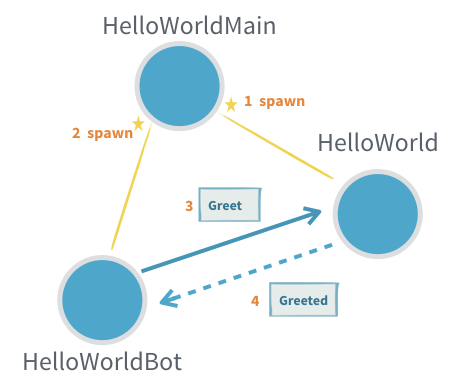
\includegraphics[width=0.7\linewidth]{images/4_state_transition}
	\caption{Übergang von Zuständen im Raft-Algorithmus}
	\label{fig:stateTransition}
\end{figure}

Dadurch, dass Akka viele wichtige Bausteine für den Aufbau verteilter Systeme auf Mikroebene (automatische Serialisierung und Deserialisierung von Nachrichten, Timers, Austausch von Behaviors) und Makroebene (Protokollunabhängigkeit, Unterstützung verteilter Aktoren und Clusters von Aktoren) bietet, ist es für die Implementierung eines verteilten Systems besonders gut geeignet.

\subsection{Einschränkungen bei der Implementierung eines verteilten Systems mit Akka}

Wie es schon im zweiten Kapitel festgestellt wurde, folgt das Aktorsystem dem Prinzip \textit{"let it crash"}, bei dem ein Kindknoten seinem Elternknoten über Ausnahmesituationen Bescheid gibt, sodass der letzte Knoten alle dieser Situationen auflöst. Wenn ein Elternknoten eine Ausnahmesituation nicht auflösen kann, delegiert er seinem Elternknoten die Verantwortung für die Situation. Dadurch entsteht ein Baum von Aktoren, in dem ein übergeordneter Knoten einen untergeordnete Knoten beobachtet und verwaltet. Das bedeutet, dass alle fehlerhaften Operationen in Blättern des \textit{Observation-Tree} (Beobachtungsbaum) konzentriert werden. Je näher ein Aktor der Wurzel des Baumes ist, desto weniger Ausnahmesituationen werden für ihn möglich sein. Die Robustheit der Hierarchie wird durch die Abgrenzung von fehlerhaften Operationen in mehreren kleinen Blattaktoren erreicht. Das stimmt mit dem bekannten Zitat des Erfinders des Aktorsystems Tony Hoare überein:

"There are two ways of constructing a software design: One way is to make it so simple that there are obviously no deficiencies and the other way is to make it so complicated that there are no obvious deficiencies."

Das Konzept der Verschiebung des kritischen Codes in äußere Knoten des Baumes nennt man \textit{Error-Kernel} (der Kernel der Fehler).

Bei Aktorsystemen ist es untypisch, wenn eine Hierarchie weniger als zwei oder drei Schichten enthält. Für eine Drohne könnte eine Hierarchie so ausschauen, wie es in der Abbildung \ref{fig:hierarchy1} dargestellt wird.

\begin{figure}
	\centering
	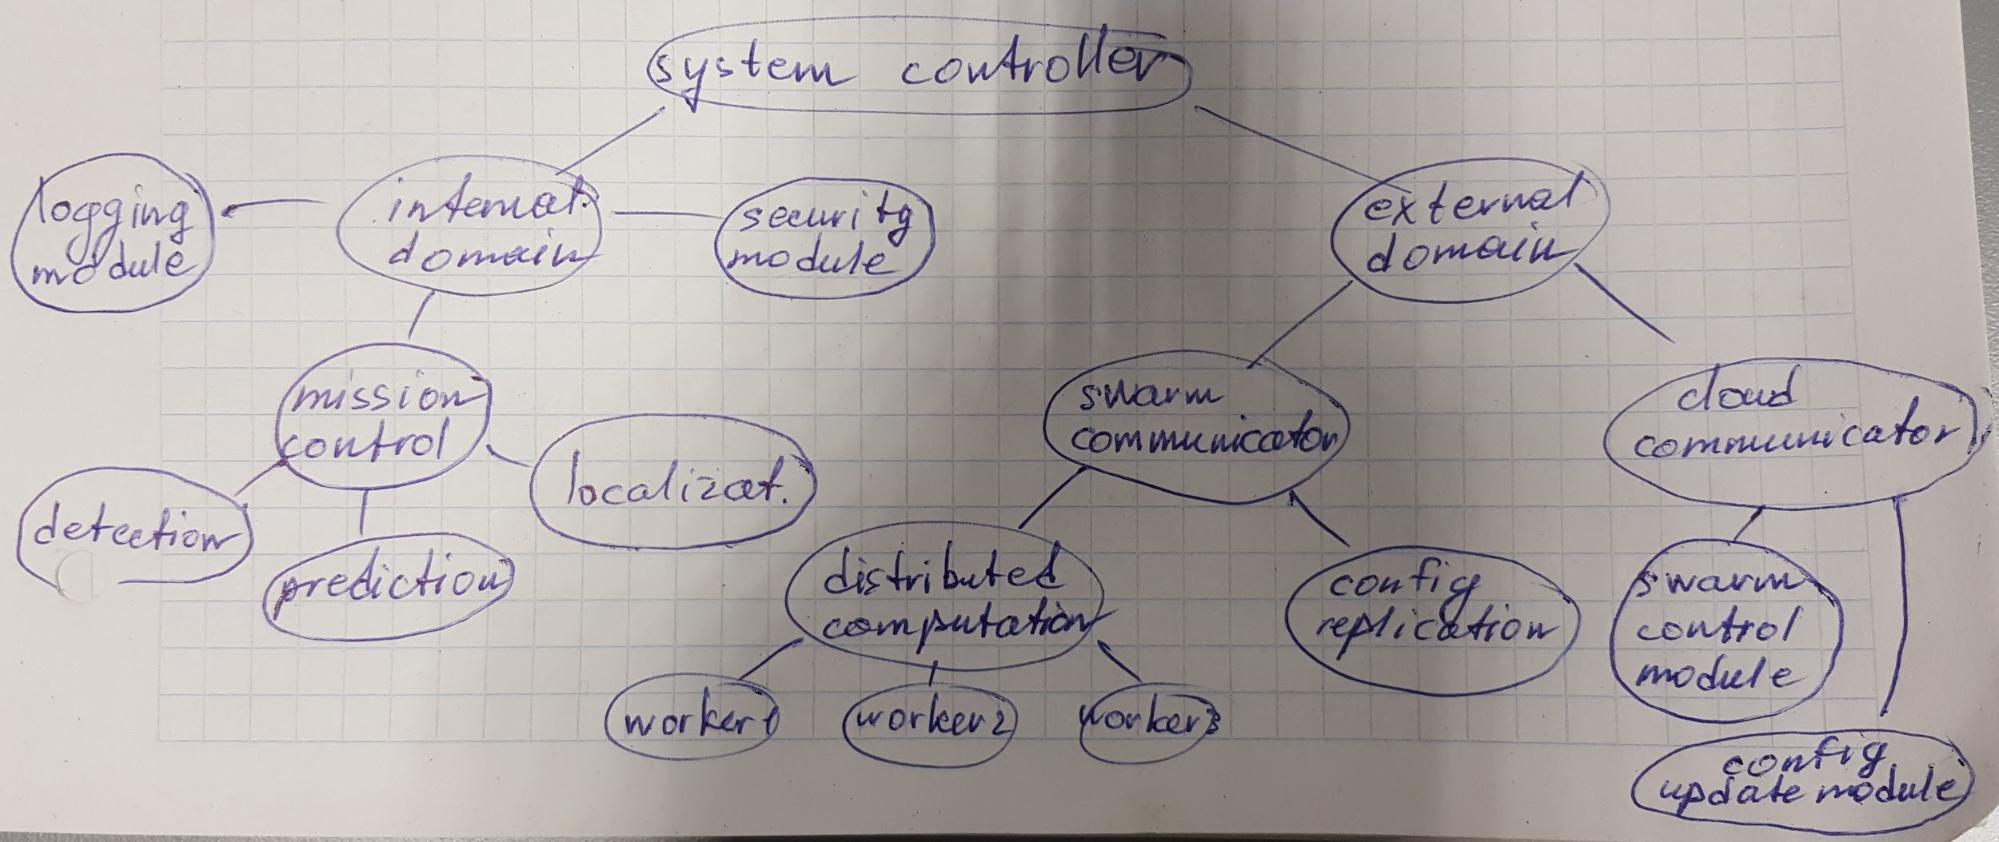
\includegraphics[width=0.7\linewidth]{images/5_hierarchy_1}
	\caption{Möglicher Aufbau eines Systems für Drohnensteuerung mithilfe Aktorsystems.}
	\label{fig:hierarchy1}
\end{figure}

Der Knoten, der für die Replikation des Zustandes zwischen den Drohnen verantwortlich ist und den Raft-Algorithmus implementiert würde, wäre \textit{Configuration-Replication} (die Replikation der Konfiguration, abgbildet rechts unten). Aufgrund des Aufbaus eines Prototypen war die Hierarchie des Raft-Algorithmus flach gehalten und nur mit zwei Schichten implementiert: eine Schicht des Clients, der Anfragen an das System entgegennimmt, und die andere Schicht der Raft Knoten. Die Hierarchie entspricht der Abbildung \ref{fig:hierarchy2}.

\begin{figure}
	\centering
	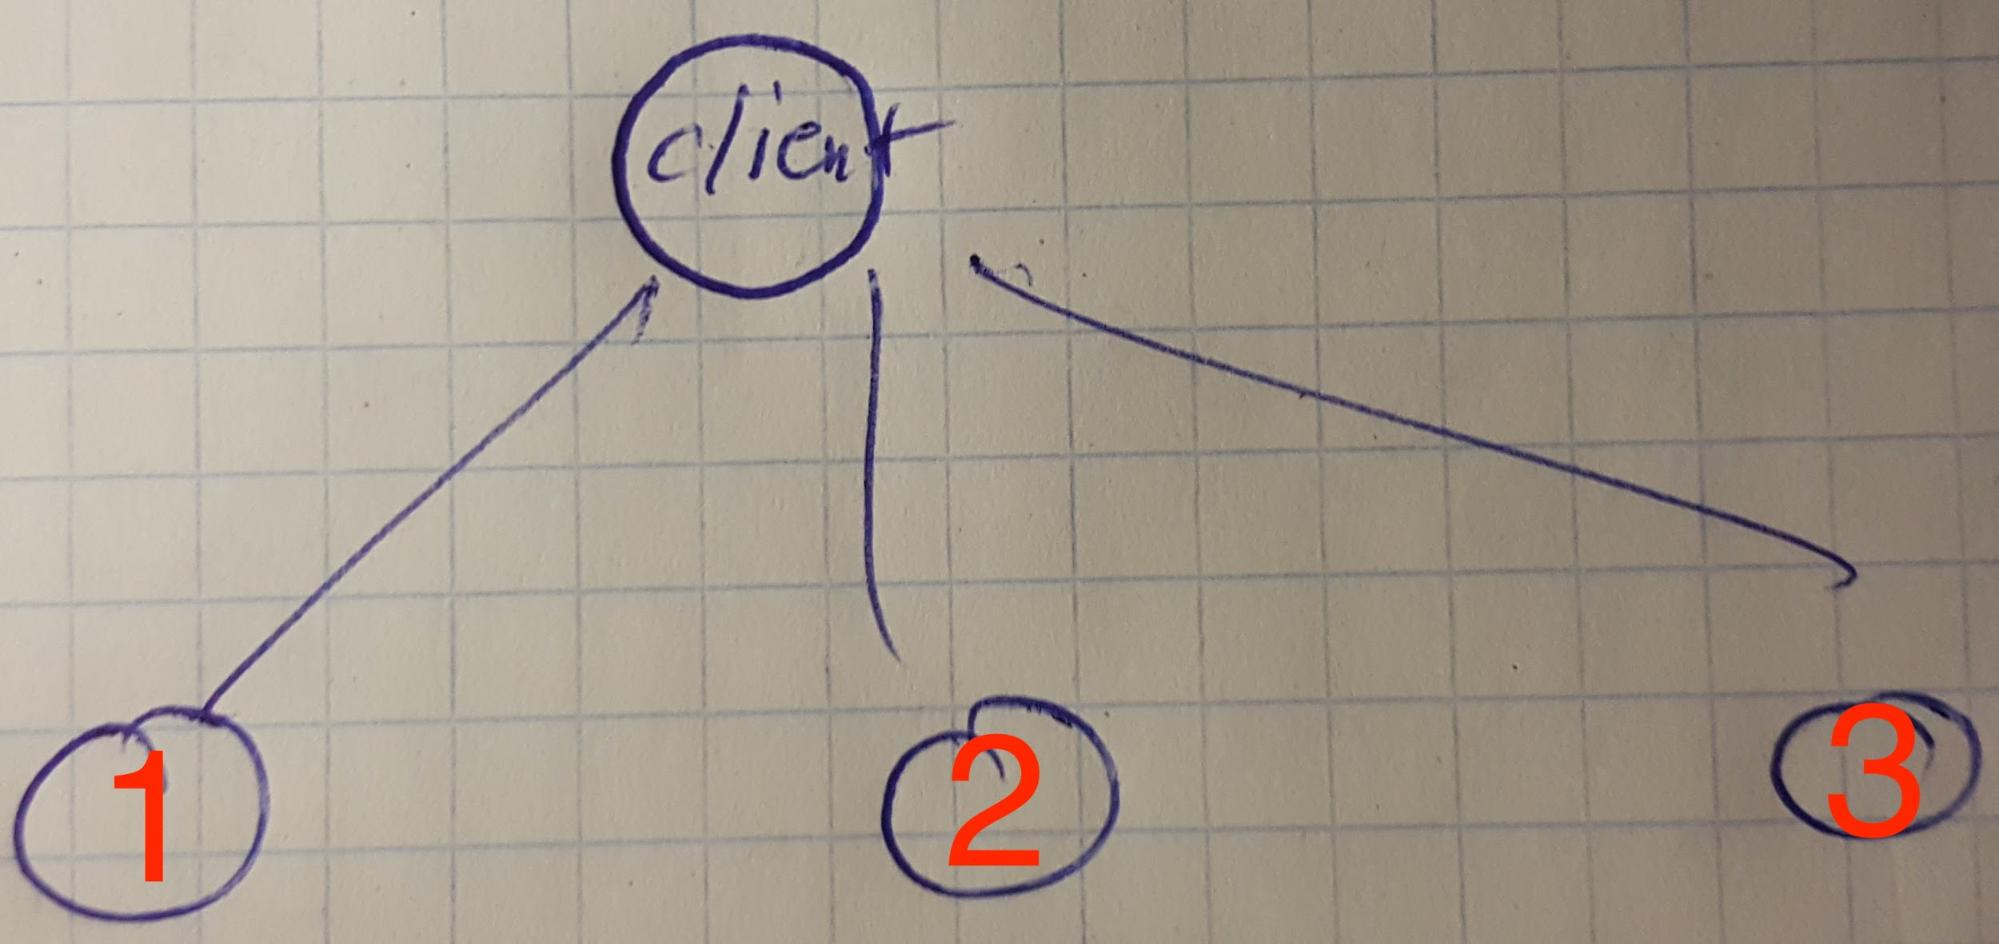
\includegraphics[width=0.7\linewidth]{images/6_hierarchy_2}
	\caption{Möglicher Aufbau eines Systems für Drohnensteuerung mithilfe Aktorsystems.}
	\label{fig:hierarchy2}
\end{figure}

Die Knoten 1, 2 und 3 entsprechen den Configuration-Replication-Knoten der ersten drei Drohnen. Der Client ist der Knoten, der sich in der Cloud befindet und als Proxy für den Drohnenschwarm dient. Der zu replizierende Wert wird vom Client an einen Knoten geschickt, der die Leader-Rolle im Cluster erfüllt und dann anschließend ohne Beteiligung des Clients laut Raft-Algorithmus zwischen Knoten repliziert.

\subsection{Annahmen für Server und Frontend des Prototypen}

Heutzutage werden vor allem zwei Frameworks für die Entwicklung von Webdiensten auf der JVM verwendet: Jakarta EE und Spring. Scala bietet ein eigenes Framework namens Play. Dies ist für die Entwicklung von  MVC- (Model View Controller) und REST-Diensten (Representational State Transfer) geeignet. Play beruht auf Akka-HTTP. Akka-HTTP ist kein Webframework, sondern ein allgemeines Werkzeug in der Akka Werkzeugpalette, um HTTP basierte Dienste aufrufen und HTTP-Anfragen beantworten zu können.

Play bietet folgende Vorteile:

\begin{enumerate}
	\item standardmäßige Unterstützung von Scala
	
	\item einfache integration mit Akka Aktorsystem
\end{enumerate}

Für die Entwicklung des Frontends wurde React verwendet. React ist ein Framework von Facebook, das eine schnelle (im Vergleich mit reinen JavaScript und HTML) Entwicklung von Webanwendungen ermöglicht.

\section{Beschreibung der Teilkomponenten und Schnittstellen des Systems}

Betrachtet man den entwickelten Prototypen abstrakt, kann er auf drei Bestandteile reduziert werden: das Frontend, das Backend und das Aktorsystem (sehe Abbildung \ref{fig:system}).

\begin{figure}
	\centering
	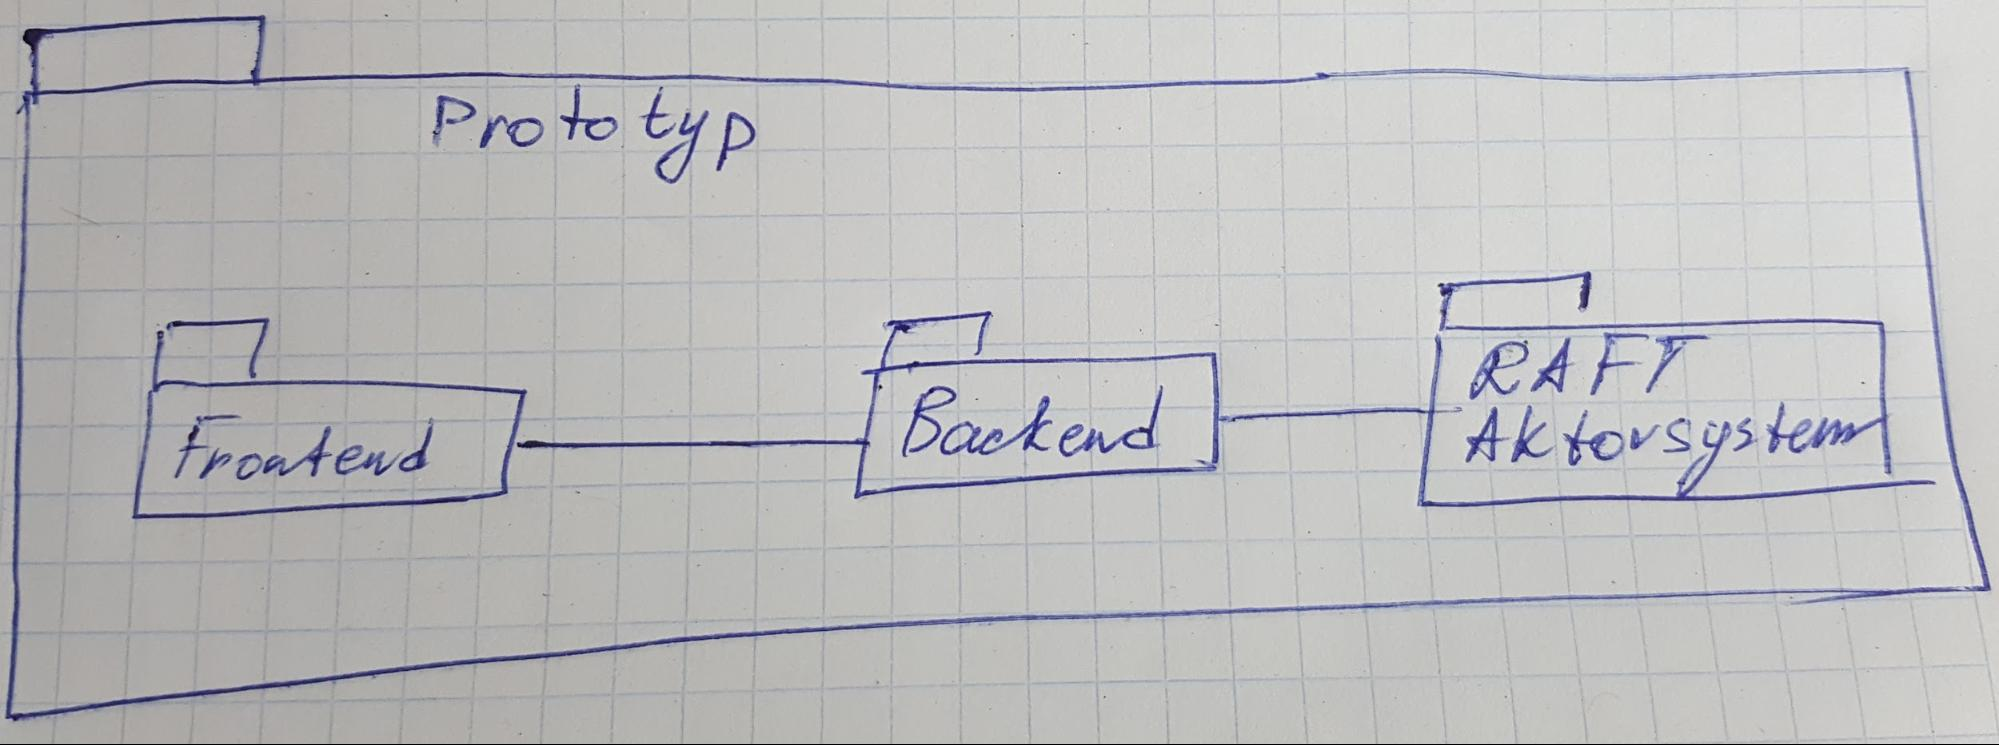
\includegraphics[width=0.7\linewidth]{images/7_system}
	\caption{Teile des Systems.}
	\label{fig:system}
\end{figure}

Das Aktorsystem wurde separat dargestellt, um zu betonen, dass das Aktorsystem eine wichtige und stichhaltige Komponente repräsentiert. Während des Entwicklungsprozesses war diese Ansicht auch dadurch gestützt, dass das Aktorsystem in einem separaten Projekt implementiert wurde. Frontend und Backend wurden ebenfalls in eigenen Projekten implementiert.

Der Prototyp verfügt über mehrere Schnittstellen. Sowohl zwischen den \textit{High-Level-Komponenten} als auch zwischen den \textit{Low-Level-Komponenten}. Zuerst werden die Schnittstellen zwischen den High-Level-Komponenten betrachtet.

\subsection{Schnittstellen zwischen High-Level-Komponenten}

Da es im Prototyp unter den High-Level-Komponenten drei Teile gibt, ergeben sich zwei Schnittstellen:

\begin{enumerate}
	\item Frontend-Backend Schnittstelle
	
	\item Backend-Aktorsystem Schnittstelle
\end{enumerate}

Die Frontend-Backend Schnittstelle ist eine REST-Schnittstelle. Frontend schickt HTTP-Anfragen an die Backend-Endpoints. Die Endpoints sind in der Tabelle \ref{tab:rest} aufgelistet.

\begin{table} \centering
	\begin{tabular}{|P{2cm}|P{2cm}|P{3cm}|P{7cm}|} 
		\hline
		\textbf{Name} & \textbf{Methode} & \textbf{Pfad} & \textbf{Beschreibung}\\
		
		\hline
		Zustand des Clusters & GET & /cluster/state & Abfrage des Zustandes eines Raft-Clusters. Die resultierende \textit{JSON-String} enthielt Informationen über einen Leader, die Followers und die Kandidaten. Diese Informationen umfassen unter anderem den Zustand des Logs, den Commit-Index (der Index des zuletzt replizierten Logeintrags) und die Nummer des aktuellen Terms.\\
		
		\hline
		Ein neues Element replizieren & POST & /cluster/item & Der Befehl speichert den Wert auf dem Cluster und liefert den aktuellen Zustand des Leader-Logs, wenn der Wert erfolgreich repliziert wurde.\\
		
		\hline
	\end{tabular}
	\caption{Endpoints der Frontend-Backend Schnittstelle.}
	\label{tab:rest}
\end{table}

Die Deklaration der oben erwähnten Endpoints ist in der \textit{routes}-Datei und die Implementierung im \textit{ClusterController} zu finden. Der ClusterController benutzt \textit{ClusterService}, um die Kommunikation zwischen dem Controller und dem Raft-Aktorsystem zu abstrahieren.

Zusätzlich befasst sich der ClusterService mit der Initialisierung des Aktorsystems. Die Initialisierung umfasst folgende Schritte:

\begin{enumerate}
	\item Erstellung von Promises und Futures
	
	\item Erstellung des Aktorsystems. Dabei wird der ClientActor als Root Aktor erstellt.
	
	\item Absenden der ClientStart-Nachricht an das System
\end{enumerate}

Futures sind Kommunikationsschnittstellen, die Ergebnisse an den ClusterService zurückgeben. Eine naheliegende Lösung wäre, anstatt eines Futures eine Callback-Funktion zu verwenden und alle Ergebnisse in diese Funktion zu übergeben. Dies hätte allerdings dem funktionalen Stil von Scala widersprochen. Deswegen wurde die Entscheidung getroffen, Futures zu verwenden. Die Futures, die in Scala verwendet werden, sind dennoch in ihrer eigenen Art herausfordernd:

\begin{description} 
	\item[Wiederverwendung von Futures.] Bei der Planung des Prototypen wurde die Entscheidung getroffen, dass es zu verschwenderisch sei, für jede Nachricht, die an das Aktorsystem geschickt wird, ein neues Promise und ein neues Future zu erstellen.
	
	\item[Timeouts.] Wenn der Zustand des Clusters abgefragt sein muss, schickt der ClusterService Anfragen an das Aktorsystem, um den aktuellen Stand des Leader, Followers und Kandidaten zu erhalten. Am Start des Clusters kann es vorkommen, dass der Zustand dann abgefragt wird, wenn es im Cluster z.B. noch keinen Leader oder keine Kandidaten gibt. In dieser Situation wäre die Zeit der Zustellung eines Ergebnisses undefiniert und unbegrenzt.
\end{description}

Um diese Herausforderungen zu meistern, wurden \textit{ReentrantPromise} und \textit{ReentrantFuture} erstellt. Die beiden Namen wurden analog zum \textit{ReentrantLock} in Java ausgewählt, um die Wiederverwendbarkeit der Instanzen dieser Klasse hervorzuheben.

ReentrantPromise setzt die Ergebnisse der asynchronen Operationen und ReentrantFuture erlaubt es, diese Ergebnisse mehrmals abzufragen. Das Ergebnis eines standardmäßigen Futures darf nur einmal aufgerufen werden. Wenn das Ergebnis eines Futures zum zweiten Mal abgefragt wird, wird eine Exception ausgelöst. Dies ist ein Schutzmechanismus, um eine unendliche Blockierung des aufrufenden Threads zu vermeiden, wenn das Ergebnis mehr als einmal abgefragt wird.

Die in Scala definierten Futures erlauben es auch nicht ein Timeout bei der Abfrage des Ergebnisses zu setzen. Eine lange Wartezeit ist für benutzerorientierte Services nicht wünschenswert. Um das zu verhindern, wurde im ReentrantFuture eine Methode mit einem Timeout als Übergabewert zum Abfragen des Ergebnisses hinzugefügt. Wenn innerhalb eines Timeouts kein Ergebnis zur Verfügung steht, wird ein leeres Ergebnis zurückgegeben.

Mittels ReentrantFutures werden folgende Informationen aus dem Aktorsystem geliefert:

\begin{enumerate}
	\item Zustand des jeweiligen Leaders
	
	\item eine Liste von Zuständen jedes Followers
	
	\item eine Liste von Zuständen jedes Kandidaten
	
	\item Zustand des Leader-Logs, nachdem ein neues Element im Cluster repliziert wurde
\end{enumerate}

Futures werden im Aktorsystem für die Zustellung der Ergebnisse alle Operationen verwendet. Um diese Operationen zu starten, müssen Nachrichten an das System geschickt werden. Beschreibung verwendeter Nachrichten findet man in Tabelle \ref{tab:operations}.

\begin{table} \centering
	\begin{tabular}{|p{5cm}|p{5cm}|p{5cm}|} 
		\hline
		\textbf{Name der Nachricht} & \textbf{Beschreibung} & \textbf{Parameter} \\
		
		\hline
		ClientStart & Da kein Discovery-System für Aktoren implementiert wurde, startet diese Nachricht ein manuelles Discovery Verfahren. & keine\\

		\hline
		Leader.Debug.InfoRequest & Den Zustand des Leaders abfragen, sofern es einen gibt. & replyTo - der Aktor, an den das Ergebnis zugestellt sein muss.\\
		
		\hline
		Candidate.Debug.InfoRequest & Den Zustand der Kandidaten abfragen. & replyTo - der Aktor, an den das Ergebnis zugestellt sein muss.\\
		
		\hline
		Follower.Debug.InfoRequest & Den Zustand der Follower abfragen. & nodeId - Id des Knoten, der Abgefragt sein muss.
		
		replyTo - der Aktor, an den das Ergebnis zugestellt sein muss.\\
		
		\hline
		ClientRequest & Einen Wert auf dem Cluster replizieren. & value - der zu replizierende Wert.
		
		replyTo - der Aktor, an den das Ergebnis zugestellt sein muss.\\
				
		\hline
	\end{tabular}
	\caption{Beschreibung der Nachrichten zur Kommunikation mit dem Aktorsystem.}
	\label{tab:operations}
\end{table}

Der Aktor, an den das Ergebnis zugestellt wird, ist immer der Client-Aktor. Dieser setzt das Ergebnis als Ergebnis des jeweiligen Promises. Promise liefert das Ergebnis mittels Thread-Synchronisation an Future, sofern das Timeout bei der Abfrage des Ergebnisses noch nicht abgelaufen ist. Das Ergebnis wird vom ClusterService erhalten und an Frontend geschickt.

\section{Kommunikationsprotokoll zwischen den Teilkomponenten und den Knoten in Raft}

Der erste Schritt bei der Implementierung des Raft-Algorithmus hat eine sorgfältige Analyse des Originalartikels erfordert. Obwohl auf Seite 4 des Raft-Artikels eine Zusammenfassung aller Rollen, Nachrichten und Feinheiten der Verhalten dargestellt wird, sind zusätzliche Informationen und Feinheiten im gesamten Artikel zu finden. Im nächsten Schritt waren alle Feinheiten nach den Rollen des Algorithmus gruppiert und in drei Tabellen entsprechend zusammengefasst.

\subsection{Definition des Followers in Raft}

Der Follower ist ein passiver Knoten in Raft und reagiert nur auf die Anfragen des Leaders und der Kandidaten. Jeder Knoten im Cluster startet im Followerzustand und setzt sofort einen Heartbeat-Timer. Wenn der Timer abläuft und sich noch kein einziger Leader gemeldet hat, wird er zum Kandidaten. Der Übergang in eine neue Rolle wird durch die Verwendung von Akka-Behaviors erreicht. Die Liste von Nachrichten, die ein Knoten in dieser Rolle empfangen kann, ist in der Tabelle \ref{tab:followerReceive} dargestellt.

\begin{table} \centering
	\begin{tabular}{|p{2.5cm}|p{3.5cm}|p{4cm}|p{4.5cm}|} 
		\hline
		\textbf{Name der Nachricht} & \textbf{Payload} & \textbf{Änderungen innerhalb des Knotens} & \textbf{Antwort auf diese Nachricht}\\
		
		\hline
		AppendEntries Heartbeat des Leaders & 
		- Leader-Information (Term und Akka-Referenz auf den Leader) & 
		- Heartbeat Timer zurücksetzen
		
		- wenn der Term des Leaders größer ist als der zuletzt gesehene Term, werden Information über den Leader geupdatet & keine\\
		
		\hline
		AppendEntries mit einem neuen Logeintrag & - Leader-Information
		
		- Letzter Logeintrag des Leaders
		
		- das zu replezierende Element
		
		- Leader-Commit
		
		- UUID des Logeintrags (in einer Fußnote erklären) 
		& - wenn der Term des Leader kleiner als der Term des zuletzt gesehenen Leaders ist, wird die Abarbeitung dieser Nachricht abgebrochen. Andernfalls werden weitere Schritte ausgeführt
		
		- Leader Information updaten
		
		- den letzten Logeintrag des Leaders mit dem eigenen letzten Logeintrag vergleichen. Wenn sie unterschiedlich sind, dann wird der Leader um die Zusendung des vorletzten Eintrags gebeten und weitere Schritte werden nicht ausgeführt. Wenn sie gleich sind, wird der Eintrag an den eigenen 
		 & - ein nicht erfolgreicher AppendEntriesResponse, um dem Leader darauf hinzuweisen, dass er diesem Knoten bisherige Logeinträge senden soll
		 
		 - ein erfolgreicher AppendEntriesResponse mit dem UUID des neuen Elements, wenn ein neuer Logeintrag an den lokalen Log angehängt wurde. Ein UUID hilft dem Leader zu identifizieren, welche Einträge und wie vielen Knoten schon erfolgreich repliziert wurden\\
		
		\hline
	\end{tabular}
	\caption{Nachrichten, die ein Follower im Raft-Algorithmus empfangen kann.}
	\label{tab:followerReceive}
\end{table}

\subsection{Definition des Kandidaten in Raft}

Die Übergangsrollen spielen in Raft die Kandidaten. Jeder Follower, dessen Heartbeat-Timer abgelaufen ist, kann zum Kandidaten werden. Der Erfolg des jeweiligen Kandidaten hängt hauptsächlich davon ab, wie kurz sein Heartbeat Timeout ist.

Nach dem Übergang von einem Follower- in einen Kandidatenzustand, startet der Kandidat einen Election-Timer (Wahl-Timer). Wenn innerhalb der Election-Zeit der Kandidat nicht zum Leader wird oder kein anderer Leader sich mit einer AppendEntries Nachricht meldet, beginnt die nächste Runde des Wahlprozesses. Alle anderen Veränderungen im Zustand eines Kandidaten werden durch empfangene und gesendete Nachricht eingeleitet, die in Tabellen \ref{tab:candidateReceive} bzw. \ref{tab:candidateSend} abgebildet sind.

\begin{table} \centering
	\begin{tabular}{|p{2.5cm}|p{3.5cm}|p{4cm}|p{4.5cm}|} 
		\hline
		\textbf{Name der Nachricht} & \textbf{Payload} & \textbf{Änderungen innerhalb des Knotens} & \textbf{Antwort auf diese Nachricht}\\
		
		\hline
		VoteGranted & kein & - Die Anzahl von Stimmen um 1 inkrementieren
		
		- Checken, ob Stimmen schon vom Quorum aller Knoten empfangen wurden. Wenn es der Fall ist, dann zum Leader werden
		 & keine\\
		
		\hline
		AppendEntries & - Leader-Information (Term und Akka-Referenz auf den Leader) 
		& - Wenn der Term des Leader größer oder gleich dem Kandidaten-Term ist, dann zum Leader werden & keine\\
		
		\hline
	\end{tabular}
	\caption{Nachrichten, die ein Kandidat empfangen kann.}
	\label{tab:candidateReceive}
\end{table}

\begin{table} \centering
	\begin{tabular}{|p{2.5cm}|p{3.5cm}|p{4cm}|p{4.5cm}|} 
		\hline
		\textbf{Name der Nachricht} & \textbf{Payload} & \textbf{Änderungen innerhalb des Knotens} & \textbf{Antwort auf diese Nachricht}\\
		
		\hline
		RequestVote & - Term des Kandidaten
		
		- Akka-Referenz auf den Kandidaten
		
		- Der letzte Logeintrag
		 & Am Start jedes Wahlprozesses & An alle Knoten im Cluster unabhängig von ihren Rollen\\
		
		\hline
	\end{tabular}
	\caption{Nachrichten, die ein Kandidat aussenden kann.}
	\label{tab:candidateSend}
\end{table}

\subsection{Definition des Leaders in Raft}

Der Leader in Raft ist der \textit{Garant des Konsenses} und spielt eine zentrale Rolle. Alle Schreiboperationen erfolgen über den Leader, der dazu noch das Replikationsverfahren steuert und alle Followers am aktuellen Stand hält. Ein Leader existiert innerhalb eines Terms und der Term endet gleich nach dem Absturz des Leaders.

Nachdem ein Kandidat die Wahl gewonnen hat und zum Leader geworden ist, etabliert er sein Leadership durch die erste Heartbeat-Nachricht, die an alle Knoten geschickt wird. Die Heartbeat-Nachricht muss der Leader regelmäßig aussenden, sodass Followers wissen, dass der Leader noch existiert. Deswegen setzt er einen Timer und schickt die Nachricht alle N Sekunden. Diese Zeit N muss unbedingt kleiner sein als die Zeit des Election-Timers eines Followers. Wenn das nicht der Fall ist, werden Followers immer schneller entscheiden, dass der Leader abgestürzt oder nicht mehr erreichbar ist. Unter diesen Umständen kann ein Leader nie ausgewählt werden.

Der Leader ist eine Schnittstelle zwischen Clients und dem Rest des Clusters. Die Nachrichten, die ein Leader aussendet und erhält, sind in Tabellen \ref{tab:leaderReceive} und \ref{tab:leaderSend} aufgelistet.

\begin{table} \centering
	\begin{tabular}{|P{2.5cm}|p{3.5cm}|p{4cm}|p{4.5cm}|} 
		\hline
		\textbf{Name der Nachricht} & \textbf{Payload} & \textbf{Änderungen innerhalb des Knotens} & \textbf{Antwort auf diese Nachricht}\\
		
		\hline
		ClientRequest 
		&
		- Der zu replizierende Wert
		
		- Die Adresse der Knoten, an den das Ergebnis der Replikation geschickt werden muss
		& 
		- Einen neuen Eintrag an eigenen Log anhängen
		
		- Den neuen Logeintrag auch in die Pending-Item Liste einfügen. Diese Liste enthält Informationen, auf wie vielen Knoten ein Logeintrag schon repliziert wurde.
		
		- Eine Append-Entries Nachricht an alle Knoten im Cluster aussenden. So eine Nachricht fungiert auch als ein Heartbeat.
		 & keine\\
		 
		 \hline
		 AppendEntriesResponse 
		 &
		 - Ein boolescher Wert, der zeigt, ob ein Wert auf einem Knoten erfolgreich / nicht erfolgreich repliziert wurde.
		 
		 - UUID des Logeintrags in der PendingItems Liste
		 
		 - Akka-Referenz auf den Follower, der diese Nachricht geschickt hat
		 & 
		 - Wenn ein Wert nicht erfolgreich repliziert wurde, dann ist der Log des Followers immer noch im inkonsistenten Zustand. Man muss 1 von NextIndex subtrahieren und versuchen, den Logeintrag vor dem NextIndex an den Follower zu schicken
		 
		 - Wenn ein Wert erfolgreich repliziert wurde, checken, ob das schon beim ersten Versuch erfolgreich war. In diesem Fall muss UUID des Eintrags in PendingItem in der Nachricht vorhanden sein.
		 
		 - Wenn ein Wert erfolgreich repliziert wurde aber UUID nicht da ist, dann ist es ein Follower, dessen Log immer noch nicht konsistent ist. Follower bittet um Zusendung des nächsten Logeintrags.
		 & 
		 - Wenn ein Wert nicht erfolgreich repliziert wurde, dann AppendEntries mit dem vorherigen Logeintrag schicken
		 
		 - Wenn der Wert auf ein Quorum repliziert wurde, Client-Response Nachricht mit dem aktuellen Stand des Zustandsautomaten zurück an den Client schicken
		 
		 - Wenn ein Logeintrag bei einem Follower mit dem inkonsistenten Log erfolgreich repliziert wurde, dann AppendEntries mit dem nächsten Logeintrag schicken\\
		 
		 \hline
		 AppendEntriesResponse 
		 &
		 
		 & 
		 
		 & keine\\
		
		\hline
	\end{tabular}
	\caption{Nachrichten, die ein Kandidat aussenden kann.}
	\label{tab:leaderReceive}
\end{table}

\begin{table} \centering
	\begin{tabular}{|p{2.5cm}|p{3.5cm}|p{4cm}|p{4.5cm}|} 
		\hline
		\textbf{Name der Nachricht} & \textbf{Payload} & \textbf{Änderungen innerhalb des Knotens} & \textbf{Antwort auf diese Nachricht}\\
		
		\hline
		Heartbeat 
		&
		- Leader-Information
		
		- Leader-Commit. Es zeigt den Index des letzten Logeintrags, den Leader commited hat.
		& 
		Regelmäßig, wenn Leader Timer abläuft
		& An alle Knoten im Cluster, unabhängig von ihren Rollen\\
		
		\hline
	\end{tabular}
	\caption{Nachrichten, die ein Leader aussenden kann.}
	\label{tab:leaderSend}
\end{table}

Bei der AppendEntries-Response Nachricht wurde \textit{NextIndex} erwähnt. NextIndex ist ein Map, das Followerreferenzen auf den nächsten Index im Log abbildet. Der jeweilige Follower erwartet diesen Index. Der Leader hält das Map im aktuellen Zustand, um zu wissen, welcher Logeintrag für welchen Follower zu einem Zeitpunkt zugeschickt sein muss, und um sicher zu stellen, dass jeder Logeintrag genau einmal zugeschickt wird. Es entspricht der \textit{"exactly once"} Nachrichtenzustellungssemantik in verteilten Systemen. Das heißt, die Nachricht darf nicht verloren gehen und darf auch nicht zweimal zugestellt werden.

\section{Besonderheiten bei der Implementierung des Raft-Algorithmus}

Bei der Implementierung des Raft-Algorithmus sind folgende Herausforderungen aufgetreten:

\begin{description} 
	\item[Tests und Absicherung.] Die Entwicklung von Komponenten eines verteilten Systems, wenn andere Komponenten noch nicht fertig oder noch in der Entwicklung sind, ist extrem schwierig. Es gibt zu viele Fakten und Feinheiten, die alle im Voraus berücksichtigt werden müssen. Weiters bereitet die asynchrone Natur der Kommunikation in verteilten Systemen (was Akka auch unterstützt) große Schwierigkeiten während des Debuggings. Deswegen wurde die Entscheidung getroffen, alle Rollen des Algorithmus und alle überschaubaren und auf den ersten Blick nicht überschaubaren Szenarien erst in Tests abzusichern und dann die getesteten Komponenten zusammenzuführen. Das Testframework für Akka-Aktoren ermöglicht eine synchrone Ausführung von Tests, während die getesteten Aktoren asynchron laufen. Das hätte viele Stunden von Debugging gekostet, wenn das ganze System ohne Tests implementiert wäre. Tests liegen im ScalaRaft Projekt in FollowerSpec, CandidateSpec bzw. LeaderSpec-Dateien.
	
	\item[Überlappungen zwischen Rollen in Raft.] Auf den ersten Blick sind alle Rollen im Raft-Algorithmus einzigartig und scheinen keine gemeinsamen Bereiche zu teilen. Bei der Implementierung ist jedoch aufgetreten, dass solche Teile, wie z.B. Discovery von Knoten, die Verwaltung des aktuellen Wertes des Zustandsautomaten, die Größe des Quorums und die Abfrage der Basisinformationen zwischen allen Rollen geteilt werden können. So ist die \textit{BaseRaftBehavior-Klasse} entstanden. Follower, Kandidat und Leader Rollen beruhen auf dieser Klasse.
	
	\item[Einschränkungen der Simulation.] Da alle Knoten des Raft-Algorithmus mit dem aktuellen Stand des Prototypen auf demselben Rechner laufen, ist es unmöglich, den Übergang eines Knotens von dem Followerzustand in den Kandidaten- und dann in Leaderzustand zu beobachten. Alle Knoten laufen lokal und den Übergang von einem Zustand in den anderen Zustand rechnet man in Millisekunden, weil alle lokal geschickte Nachrichten durch geteilte Teile des Arbeitsspeichers zugestellt werden.
	
	\item[Pending Items.] Eine offene Frage während der Implementierung gab es für die Weise, auf die noch nicht replizierte Logeinträge auf dem Leader Knoten gespeichert werden. Im Raft Artikel steht dafür nur:
	\\
	\\
	"A log entry is committed once the leader that created the entry has replicated it on a majority of the servers"
	\\
	\\
	ohne irgendwelcher Hinweise auf Implementierungsdetails. Deswegen war folgende Lösung umgesetzt. Leader führt ein Map mit allen Logeinträgen, die noch nicht repliziert wurden. Schlüssel bei diesem Map ist UUID und Wert ist PendingItem Eintrag. PendingItem enthielt Logeintrag selber, Replikationszähler für die Anzahl von Knoten, auf denen der Eintrag schon repliziert wurde, und Akka-Referenz auf den Client, der auf Ergebnis wartet. Wenn ein Follower den Eintrag erfolgreich repliziert, schickt er AppendEntriesResponse mit UUID des Pending-Eintrags. Entsprechender Pending Eintrag wird nach dem UUID aus dem Map extrahiert und Replikationszähler um 1 erhöht. Wenn Replikationszähler gleich dem Quorumgröße ist, dann wird ClinetResponse Nachricht an den Client geschickt und der Eintrag aus dem PendingItem Map gelöscht.
\end{description}

\section{Fazit}

Akka hat sich bewährt als eine saubere Lösung für Entwicklung verteilter Systeme. Mit den Werkzeugen, die Akka zur Verfügung stellt, kann man sich bei der Umsetzung des Systems nur auf das wesentliche konzentrieren, was Zeit beim Planen, Testen und Debugging erheblich spart. Andere Features von Akka, wie z.B. Akka Remoting, Akka Cluster oder Akka Sharding bringen noch mehr Möglichkeiten und Wege, Implementierung und Funktionsweise verteilter Systeme zu optimieren. Scala mit dem Pattern Matching, dem Optional Datentyp und anderen Besonderheiten stellt eine gute Option für Aufbau von Prototypen dar. Überlegungen über die Struktur des voraussichtlichen Produktivsystems bringt Basis für die nächsten Schritte bei der Entwicklung weiterer Prototypen.